\documentclass{beamer}
\usepackage{polski}
\usepackage[utf8x]{inputenc}
\usepackage{default,longtable}
\title{Wizualizacja ontologii zapisanych w języku OWL}
\author{Piotr Kunowski}
\mode<presentation>
{
\usetheme{Warsaw}
}
\begin{document}

\begin{frame}
  \titlepage
\end{frame}

\section{Motto}
\begin{frame}
\begin{block}{motto} 

"Wiedza nie wystarczy, musimy ją stosować. \\
Wola nie wystarczy, musimy działać."
\begin{flushright}
J. W. Goethe
\end{flushright}
\end{block}
 

\end{frame}


\section{Definicja problemu}

\subsection{Cel pracy}

\begin{frame}
  \frametitle{Cel pracy}
  \begin{block}{Cel}
	Celem pracy jest zaprojektowanie oraz zaimplementowanie biblioteki umożliwiającej wizualizację w przejrzysty 
sposób dowolnie złożonej ontologii zdefiniowanej w języku OWL oraz przechowywanej w postaci obiektów OWL API
  \end{block}
\end{frame}

\begin{frame}
  \frametitle{Zadania do wykonania}
  \begin{enumerate}
    \item Zapoznanie się z biblioteką Prefuse oraz porównanie jej możliwości z innymi bibliotekami służącymi do wizualizacji informacji
    \item Zapoznanie się z językiem OWL oraz z biblioteką OWL API
    \item Opracowanie graficznej reprezentacji konstrukcji dostępnych w języku OWL
    \item Opracowanie algorytmów wydajnej kompozycji symboli w graficzną reprezentację dowolnie złożonej ontologii
  \end{enumerate}

\end{frame}
\subsection{Ontologia}
\begin{frame}
  \frametitle{Ontologia - definicja}
\begin{block}{Ontologia}
Ontologia to logiczna reprezentacja pewnej dziedziny wiedzy i relacji między obiektami w niej występującymi. 
\end{block}
\end{frame}


\subsection{OWL}

\begin{frame}
  \frametitle{OWL - definicja}
 \begin{block}{OWL}
 OWL (Web Ontology Language) to język opisu ontologii (i obiektów należących do jej dziedziny) będący specyfikacją W3C, przygotowany z myślą o tworzeniu ontologii w środowisku internetowym.
\end{block}
\end{frame}

\begin{frame}
\frametitle{OWL - Lite}
 \begin{itemize}
 \item zawiera bazowe elementy OWL i RDF
	\begin{itemize}
	\item typy: Class, Property, Individual
	\item podstawowe nierówności, zależności, charakterystyki
	\item elementarna kardynalność
	\item adnotacje
\end{itemize}
\item pozwala budować hierarchię elementów
\item wymaga separacji typów
\end{itemize}
\end{frame}
\begin{frame}
\frametitle{OWL - DL}
\begin{itemize}
	\item zawiera wszystkie elementy języka OWL Lite
	\item dodatkowo zawiera zaawansowane elementy języka OWL
		\begin{itemize}
 		\item ma rozwiniętą obsługę zależności między elementami podstawowymi
		\item obsługuje kardynalność w jej pełnej formie
		\end{itemize}
	\item można go bezpośrednio mapować na logikę opisową SHOIN - jest rozstrzygalny
	\item tą wersję obsługuje portalSubsystem
	\end{itemize}

\end{frame}
\begin{frame}
\frametitle{OWL - Full}


\begin{itemize}
	\item zawiera wszystkie elementy OWL DL
	\item nie wymaga separacji typów
	\item ma mniejsze ograniczenia od OWL DL
	\item nie ma w nim gwarancji rozstrzygalności dla wnioskowań
	\end{itemize}
\end{frame}



\begin{frame}
	\frametitle{Istniejące biblioteki graficzne}
	\begin{block}{JUNG (Java Universal Network/Graph Framework)}
		\begin{itemize}
			\item	wizualizacja danych za pomocą grafów oraz sieci
			\item posiada podstawowe algorytmy grafowe
			\item BSD
	\end{itemize}
	\end{block}
	\begin{block}{JGraph}
		\begin{itemize}
			\item	 biblioteka do wizualizacji grafów kompatybilna ze Swingiem
				\item posiada podstawowe algorytmy grafowe
			\item LGPL
	\end{itemize}
	\end{block}
\end{frame}

\begin{frame}
	\frametitle{Istniejące biblioteki graficzne}
	\begin{block}{Prefuse}
		\begin{itemize}
			\item  elastyczna 
			\item narzędzia do przechowywania danych
			 \item narzędzia do manipulowania danymi 
			\item interaktywność wizualizacji 
                        \item ciągle rozwijana  
			\item BSD
			\item Wykorzystana w OCS i GrOWL     
		\end{itemize}
	\end{block}
	\begin{block}{Piccolo}
		\begin{itemize}
			\item	rozbudowany zestaw narzędzi 
			\item perspektywa rybiego oka
			\item  istnieją trzy wersje: Piccolo.Java, Piccolo.NET oraz PocketPiccolo.NET 
			\item wykorzystana w pluginie do Protege o nazwie Jambalaya
			\item BSD
	\end{itemize}
	\end{block}
\end{frame}


\begin{frame}
  \frametitle{Kryteria porównawcze}
Należy zwrócić uwagę na sposób wizualizacji następujących elementów:
\begin{itemize}
  \item Klasy i instancje \pause
  \item Hierarchia klas \pause
  \item Wielokrotne dziedziczenie \pause
  \item Relacje \pause
  \item Właściwości \pause
\end{itemize}
ponad to należy uwzględnić:
\begin{itemize}
  \item możliwość wyszukiwania i filtrowania \pause
  \item licencja \pause
\end{itemize}
\end{frame}



\section{Porównanie istniejących rozwiązań}

\begin{frame}
  \frametitle{Istniejące rozwiązania}
  \begin{itemize}
    \item OntoViv
    \item Growl
    \item Jambalaya
    \item OCS
  \end{itemize}

\end{frame}


\subsection{OntoViz}


\begin{frame}
  \frametitle{OntoViv}
  \begin{itemize}
    \item Klasy i instancje reprezentowane jako prostokątne wierzchołki grafu wyróżnione innymi kolorami
    \item Klasy pochodne znajdują się pod klasą rodzica połączone związkiem 'isa'
    \item Klasy są połączone z wszystkimi swoimi podklasami
    \item Relacja odzwierciedlana jako związek z etykietą. Brak odzwierciedlenia wszystkich relacji.
    \item Właściwości wyświetlane wewnątrz wierzchołka
    \item Brak możliwości wyszukiwania.
    \item Licencja: Mozilla Public License
  \end{itemize}

\end{frame}


\begin{frame}
  \frametitle{OntoViv}
\begin{center}
 \scalebox{0.30}{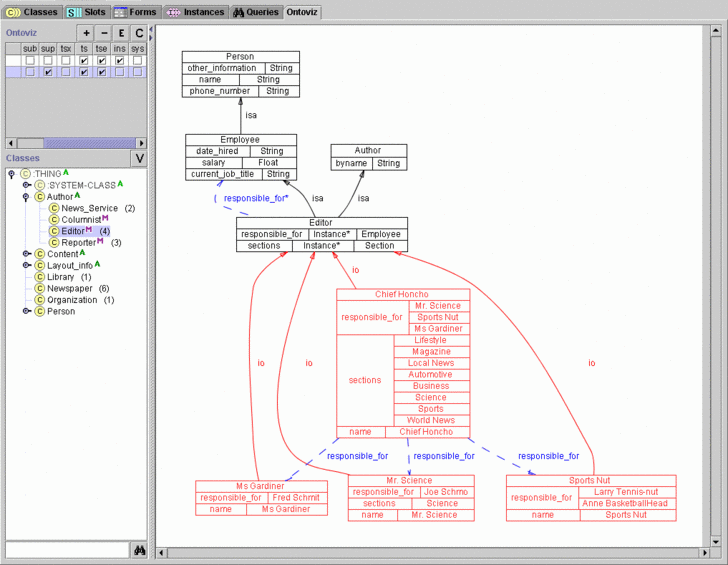
\includegraphics{./prezentacja_img/OntoViz.png}}
\end{center}
\end{frame}

\subsection{Jambalaya}
\begin{frame}
  \frametitle{Jambalaya}

  \begin{itemize}
    \item Klasy i instancje reprezentowane jako prostokąty o różnych kolorach
    \item Klasy pochodne reprezentowane są jako mniejsze prostokąty leżące wewnątrz  klasy rodzica
    \item Klasa dziedzicząca znajduję się w każdym  z prostokątów rodzica
    \item Relacja odzwierciedlana jako skierowane krawędzie. Brak odzwierciedlenia wszystkich relacji.
    \item Właściwości wyświetlane jako jedno z pół oglądanej klasy.
    \item Możliwość filtrowania i wyszukiwania.
    \item Licencja: brak danych
  \end{itemize}

\end{frame}


\begin{frame}
  \frametitle{OntoViv}
\begin{center}
 \scalebox{0.30}{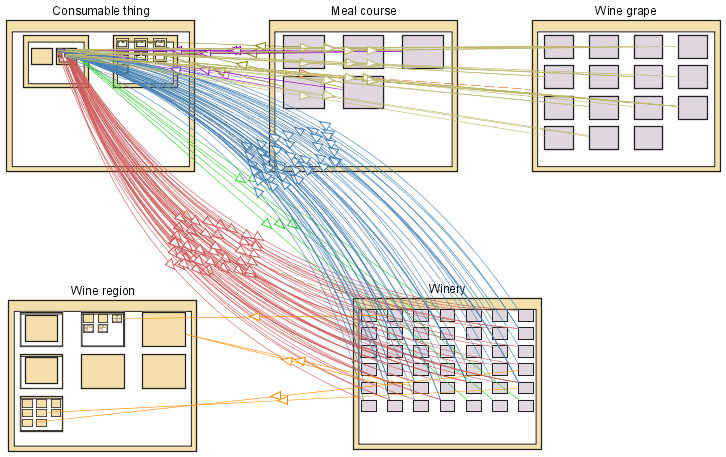
\includegraphics{./prezentacja_img/jambalaya.png}}
\end{center}
\end{frame}

\subsection{GrOWL}
\begin{frame}
  \frametitle{GrOWL}
\begin{itemize}
    \item Klasy i instancje są prostokątami o różnych kolorach w grafie
    \item Klasy pochodne połączone są z klasami nadrzędnymi skierowaną krawędzią.  
    \item Klasa dziedzicząca połączona jest ze wszystkimi nadklasami
    \item Relacja odzwierciedlana jako różnego rodzaju krawędzie, często typ relacji wskazany jest przez dodatkowy wierzchołek.
    \item Właściwości wyświetlane są jako zaokrąglone prostokąty w grafie, odpowiednio połączone z pozostałymi elementami ontologii.
    \item Możliwość filtrowania i wyszukiwania.
    \item Licencja: GPL
  \end{itemize}

\end{frame}

\begin{frame}
  \frametitle{OntoViv}
\begin{center}
 \scalebox{0.30}{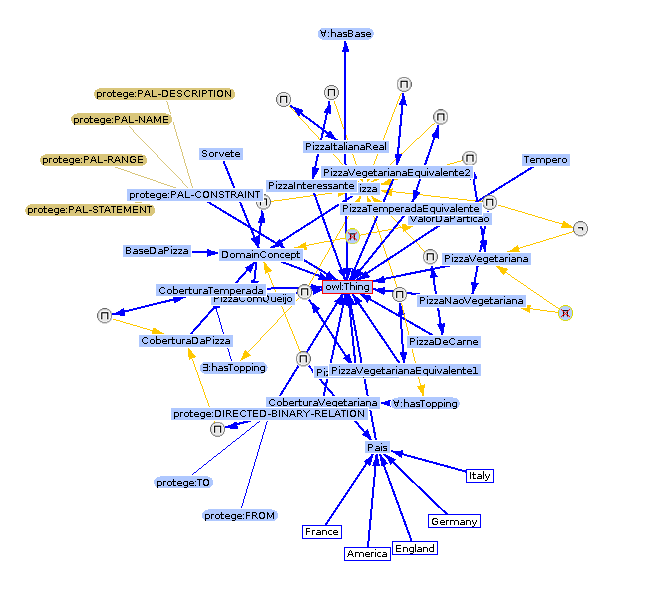
\includegraphics{./prezentacja_img/growl.png}}
\end{center}
\end{frame}


\subsection{OCS}
\begin{frame}
  \frametitle{OCS}
  \begin{itemize}
    \item Klasy wyświetlane są jako zaokrąglone prostokąty. Instancje wizualizowane są tylko w diagramie hierarchii wnioskowania, posiadają inny kolor niż klasy.
    \item Klasy pochodne połączone są z klasami nadrzędnymi związkiem subClass.  
    \item Klasa dziedzicząca połączona jest ze wszystkimi nadklasami
    \item Odzwierciedla tylko 2 typy relacji. Za pomocą strzałek z etykietą.
    \item Brak wizualizacji właściwości. 
    \item Możliwość filtrowania relacji.
    \item Licencja: ?
  \end{itemize}

\end{frame}

\begin{frame}
  \frametitle{OntoViv}
\begin{center}
 \scalebox{0.30}{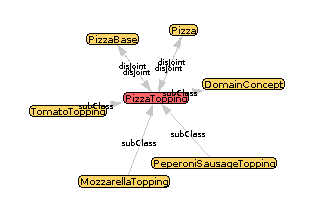
\includegraphics{./prezentacja_img/ocs1.png}}
\end{center}
\end{frame}


\section{SOVA}
\begin{frame}
	\frametitle{SOVA - czyli to co już jest}
	 \begin{block}{SOVA}
		Simple Ontology Visualization API
	\end{block} 
\end{frame}

\begin{frame}
	\frametitle{Wizualizacja elementów OWL}
	
\begin{longtable}{lp{7cm}} 

  Thing &
 \scalebox{0.30}{
\includegraphics{./elementyGraficzne/drobne/thing.png}}
 % class.png: 194x86 pixel, 90dpi, 5.48x2.43 cm, bb=0 0 155 69
 \\ 

  Nothing &
 \scalebox{0.30}{
\includegraphics{./elementyGraficzne/drobne/nothing.png}}
 % class.png: 194x86 pixel, 90dpi, 5.48x2.43 cm, bb=0 0 155 69
 \\ 

  Class &
 \scalebox{0.30}{
\includegraphics{./elementyGraficzne/drobne/class.png}}
 % class.png: 194x86 pixel, 90dpi, 5.48x2.43 cm, bb=0 0 155 69
 \\ 

  Individual &
 \scalebox{0.30}{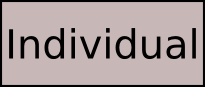
\includegraphics{./elementyGraficzne/drobne/individual.png}}
 % class.png: 194x86 pixel, 90dpi, 5.48x2.43 cm, bb=0 0 155 69
 \\ 

  Property &
 \scalebox{0.30}{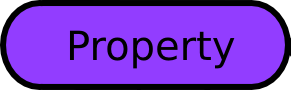
\includegraphics{./elementyGraficzne/drobne/property.png}}
 % class.png: 194x86 pixel, 90dpi, 5.48x2.43 cm, bb=0 0 155 69
 \\ 

  Datatype &
 \scalebox{0.30}{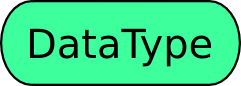
\includegraphics{./elementyGraficzne/drobne/datatype.png}}
 % class.png: 194x86 pixel, 90dpi, 5.48x2.43 cm, bb=0 0 155 69
 \\ 

  Anonymous Class &
 \scalebox{0.30}{
\includegraphics{./elementyGraficzne/drobne/anonymousClass.png}}
 % class.png: 194x86 pixel, 90dpi, 5.48x2.43 cm, bb=0 0 155 69
 \\ 

  Subclass &
 \scalebox{0.30}{
\includegraphics{./elementyGraficzne/drobne/subclass.png}}
 % class.png: 194x86 pixel, 90dpi, 5.48x2.43 cm, bb=0 0 155 69
 \\ 


\end{longtable}
\end{frame}


\begin{frame}
	\frametitle{Wizualizacja elementów OWL}
	
\begin{longtable}{lp{7cm}} 
 instanceOf &
 \scalebox{0.30}{
\includegraphics{./elementyGraficzne/drobne/instanceOf.png}} \newline
 \scalebox{0.30}{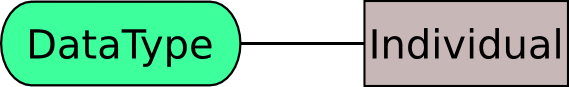
\includegraphics{./elementyGraficzne/drobne/instanceOfDatatype.png}}
 % class.png: 194x86 pixel, 90dpi, 5.48x2.43 cm, bb=0 0 155 69
 \\  

equivalentClass &
 \scalebox{0.30}{
\includegraphics{./elementyGraficzne/drobne/equivalentClass.png}}
 % class.png: 194x86 pixel, 90dpi, 5.48x2.43 cm, bb=0 0 155 69
 \\ 

  disjointWith &
 \scalebox{0.30}{
\includegraphics{./elementyGraficzne/drobne/disjointWith.png}}
 % clas.png: 194x86 pixel, 90dpi, 5.48x2.43 cm, bb=0 0 155 69
 \\ 

  differentFrom / allDifferent &
 \scalebox{0.30}{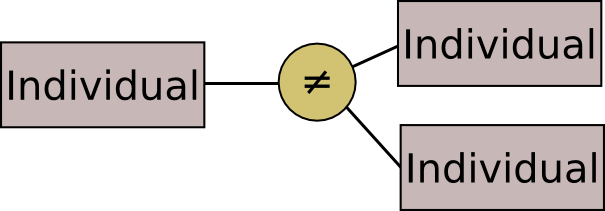
\includegraphics{./elementyGraficzne/drobne/allDifferent.png}}
 % class.png: 194x86 pixel, 90dpi, 5.48x2.43 cm, bb=0 0 155 69
 \\ 

  sameAs &
 \scalebox{0.30}{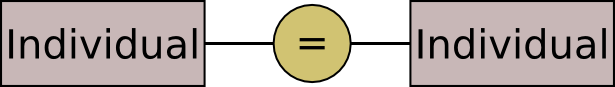
\includegraphics{./elementyGraficzne/drobne/sameAs.png}}
 % class.png: 194x86 pixel, 90dpi, 5.48x2.43 cm, bb=0 0 155 69
 \\ 

\end{longtable}
\end{frame}


\begin{frame}
	\frametitle{Wizualizacja elementów OWL}
	
\begin{longtable}{lp{7cm}} 
 

  oneOf &
 \scalebox{0.30}{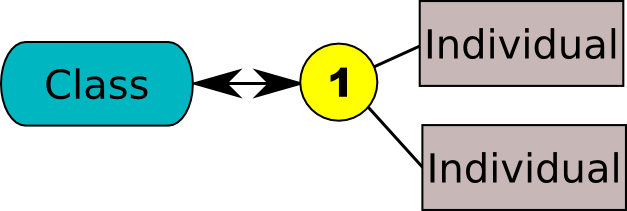
\includegraphics{./elementyGraficzne/drobne/oneOf.png}}
 % class.png: 194x86 pixel, 90dpi, 5.48x2.43 cm, bb=0 0 155 69
 \\ 

  unionOf &
 \scalebox{0.30}{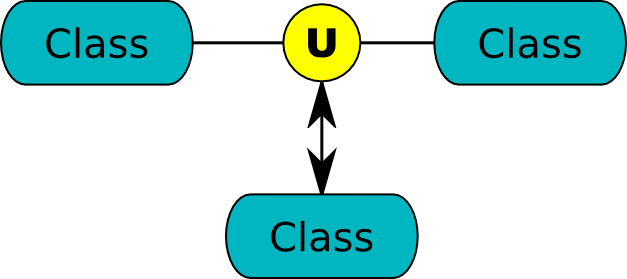
\includegraphics{./elementyGraficzne/drobne/unionOf.png}}
 % class.png: 194x86 pixel, 90dpi, 5.48x2.43 cm, bb=0 0 155 69
 \\ 

  intersectionOf &
 \scalebox{0.30}{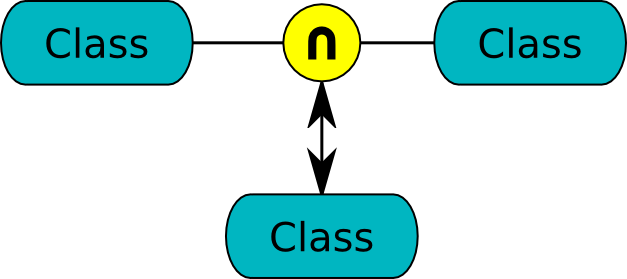
\includegraphics{./elementyGraficzne/drobne/intersectionOf.png}}
 % class.png: 194x86 pixel, 90dpi, 5.48x2.43 cm, bb=0 0 155 69
 \\ 


\end{longtable}
\end{frame}


\begin{frame}
	\frametitle{Wizualizacja elementów OWL}
	
\begin{longtable}{lp{7cm}} 
 

  complementOf &
 \scalebox{0.30}{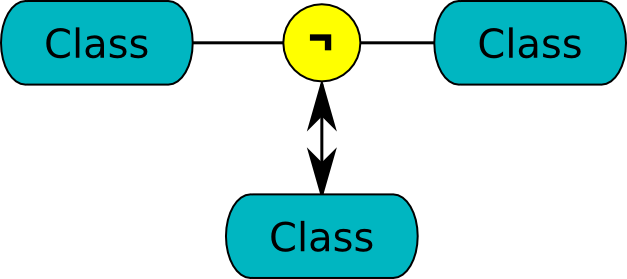
\includegraphics{./elementyGraficzne/drobne/complementOf.png}}
 % class.png: 194x86 pixel, 90dpi, 5.48x2.43 cm, bb=0 0 155 69
 \\ 

  subProperty &
 \scalebox{0.30}{
\includegraphics{./elementyGraficzne/drobne/subProperty.png}}
 % class.png: 194x86 pixel, 90dpi, 5.48x2.43 cm, bb=0 0 155 69
 \\ 

  inverseOf (property) &
 \scalebox{0.30}{
\includegraphics{./elementyGraficzne/drobne/inverseOf.png}} \newline
\scalebox{0.30}{
\includegraphics{./elementyGraficzne/drobne/inverseOfProperty.png}}
 % class.png: 194x86 pixel, 90dpi, 5.48x2.43 cm, bb=0 0 155 69
 \\ 

  equivalentProperty &
 \scalebox{0.30}{
\includegraphics{./elementyGraficzne/drobne/equivalentProperty.png}}
 % class.png: 194x86 pixel, 90dpi, 5.48x2.43 cm, bb=0 0 155 69
 \\ 

\end{longtable}
\end{frame}




\begin{frame}
	\frametitle{Wizualizacja elementów OWL}
	
\begin{longtable}{lp{7cm}} 
 
  functionalProperty &
 \scalebox{0.30}{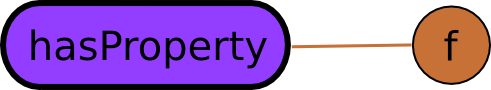
\includegraphics{./elementyGraficzne/drobne/functionalProperty.png}}
 % class.png: 194x86 pixel, 90dpi, 5.48x2.43 cm, bb=0 0 155 69
 \\ 

  inverseFunctionalProperty &
 \scalebox{0.30}{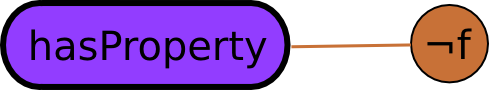
\includegraphics{./elementyGraficzne/drobne/inverseFunctionalProperty.png}}
 % class.png: 194x86 pixel, 90dpi, 5.48x2.43 cm, bb=0 0 155 69
 \\ 

  symmetricProperty &
 \scalebox{0.30}{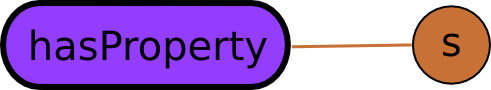
\includegraphics{./elementyGraficzne/drobne/symmetricProperty.png}}
 % class.png: 194x86 pixel, 90dpi, 5.48x2.43 cm, bb=0 0 155 69
 \\ 

  transitiveProperty &
 \scalebox{0.30}{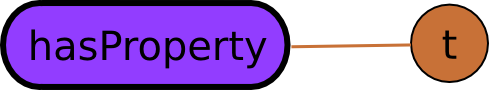
\includegraphics{./elementyGraficzne/drobne/transitiveProperty.png}}
 % class.png: 194x86 pixel, 90dpi, 5.48x2.43 cm, bb=0 0 155 69
 \\ 

  hasProperty &
 \scalebox{0.25}{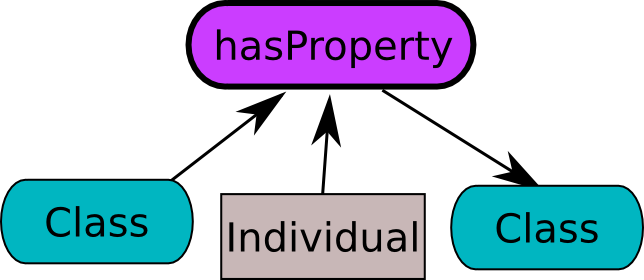
\includegraphics{./elementyGraficzne/drobne/hasProperty.png}}
 % class.png: 194x86 pixel, 90dpi, 5.48x2.43 cm, bb=0 0 155 69
 \\ 

  domain &
 \scalebox{0.25}{
\includegraphics{./elementyGraficzne/drobne/domain.png}}
 % class.png: 194x86 pixel, 90dpi, 5.48x2.43 cm, bb=0 0 155 69
 \\ 

  range &
 \scalebox{0.25}{
\includegraphics{./elementyGraficzne/drobne/range.png}}
 % class.png: 194x86 pixel, 90dpi, 5.48x2.43 cm, bb=0 0 155 69
 \\ 



\end{longtable}
\end{frame}


\begin{frame}[allowframebreaks]{Outline}

	\frametitle{Wizualizacja elementów OWL}
\begin{longtable}{lp{7cm}} 


  allValuesFrom &
 \scalebox{0.25}{
\includegraphics{./elementyGraficzne/drobne/allValuesFrom.png}}
 % class.png: 194x86 pixel, 90dpi, 5.48x2.43 cm, bb=0 0 155 69
 \\ 

  someValuesFrom &
 \scalebox{0.25}{
\includegraphics{./elementyGraficzne/drobne/someValuesFrom.png}}
 % class.png: 194x86 pixel, 90dpi, 5.48x2.43 cm, bb=0 0 155 69
 \\ 

  minCardinality / maxCardinality &
 \scalebox{0.30}{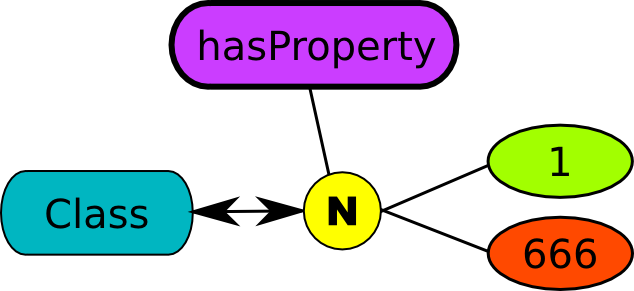
\includegraphics{./elementyGraficzne/drobne/cardinalityminmax.png}}
 % class.png: 194x86 pixel, 90dpi, 5.48x2.43 cm, bb=0 0 155 69
 \\ 

  cardinality &
 \scalebox{0.30}{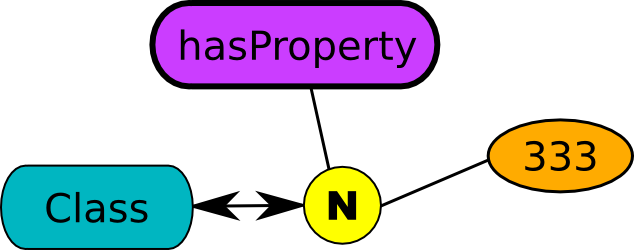
\includegraphics{./elementyGraficzne/drobne/cardinality.png}}
 % class.png: 194x86 pixel, 90dpi, 5.48x2.43 cm, bb=0 0 155 69
 \\ 


\end{longtable}
\end{frame}

\begin{frame}
  \frametitle{Literatura}
\begin{itemize}


\item Brachman, R.J. and Levesque, H.J., Knowledge Representation and Reasoning, Morgan Kaufmann, 2004
\item Grimm, S. and Hitzler, P. and Abecker, A., Knowledge Representation and Ontologies, Springer, 2007
\item Staab, S., Handbook on ontologies, Springer, 2004
\item Katifori A., Halatsis C., Lepouras G., Vassilakis C., Giannopoulou E., Ontology Visualization Methods – A Survey, ACM Computing Surveys, Vol. 39, No. 4, Article 10, 2007
\item Storey M., Lintern R., Ernst N., Perrin D., Visualization and Protégé, http://protege.stanford.edu/conference/2004/abstracts/Storey.pdf, 2004
\item Horridge M., OWLViz, http://code.google.com/p/co-ode-owl-plugins/wiki/OWLViz, 2010
\end{itemize}
\end{frame}
\begin{frame}
  \frametitle{Literatura c.d.}
\begin{itemize}

\item Stanford Center for Biomedical Informatics Research, http://protege.stanford.edu/, 2009
\item Gennari J. H., Musen M. A., Fergerson R. W., Grosso W. E., Crubézy M., Eriksson H., Noy N. F., Tu S. W.: The evolution of Protégé: An environment for knowledge-based systems development, Technical Report SMI-2002-0943, Stanford Medical Institute, 2002
\item Noy N. F., Fergerson R. W., Musen M. A.: The knowledge model of Protégé-2000: Combining interoperability and flexibility, Lecture Notes in Computer Science, Springer-Verlag, 2000
\item Krivov S., Williams R., Villa F., GrOWL: A tool for visualization and editing of OWL ontologies, Web Semantics: Science, Services and Agents on the World Wide Web , Vol 5, Issue 2, 2007, p. 54-57, 2007
\item Carroll J. J., Reynolds D., Dickinson I., Seaborne A., Dollin C., Wilkinson K., Jena: Implementing the Semantic Web Recommendations, Digital Media Systems Laboratory, HP Laboratories Bristol, HPL-2003-146, 2003
\item Boiński T., Budnik Ł., Jakowski A., Mroziński J., Mazurkiewicz K., OCS - domain oriented Ontology Creation System, Sejmik Młodych Informatyków, Polish Journal of Environmental Studies, Vol 18, No. 3B, 2009, p. 35-38, 2009
\end{itemize}
\end{frame}
\begin{frame}
  \frametitle{Literatura c.d.}
\begin{itemize}

\item W3C, Web Ontology Language (OWL), http://www.w3.org/2004/OWL/, 2004
\item Horridge M., Bechhofer S., The OWL API: A Java API for Working with OWL 2 Ontologies, 6th OWL Experienced and Directions Workshop, 2009
\item Heer J., Card S. K., Landay J. A., Prefuse: a toolkit for interactive information visualization, Proceedings of the SIGCHI conference on Human factors in computing systems, p. 421-430, Portland, Oregon, USA: ACM, 2005
\item Boiński T., Jaworska A., Kleczkowski R., Kunowski P., Ontology Visualization, 2010.
\end{itemize}
\end{frame}



\end{document}
